\section{Background}
\label{sec:background}

\par Emotions are complex experiences of consciousness, bodily sensation, and behavior that reflects the personal significance of a thing, or an event. Plutchik introduced the Wheel of Emotions, a model that identifies eight fundamental emotions: joy, sadness, trust, disgust, fear, anger, anticipation, and surprise. According to this model, these basic emotions can combine in varying intensities to form more complex emotional states. Others are overlapping those fundamental emotions which can be seen in Figure~\ref{fig:wheel}. This research is the base for upcoming research in emotion categorization \citep{plutchik1980general}. Valence-Arousal-Dominance (VAD) model represents emotions along three dimensions: pleasantness (valence), activation (arousal), and control (dominance). It provides a simple and intuitive way to understand the different components of emotion Figure~\ref{fig:two-dim}. \citep{oberlander2018analysis}.

\begin{figure*}[h]
\centering
\begin{subfigure}[b]{0.45\textwidth}
    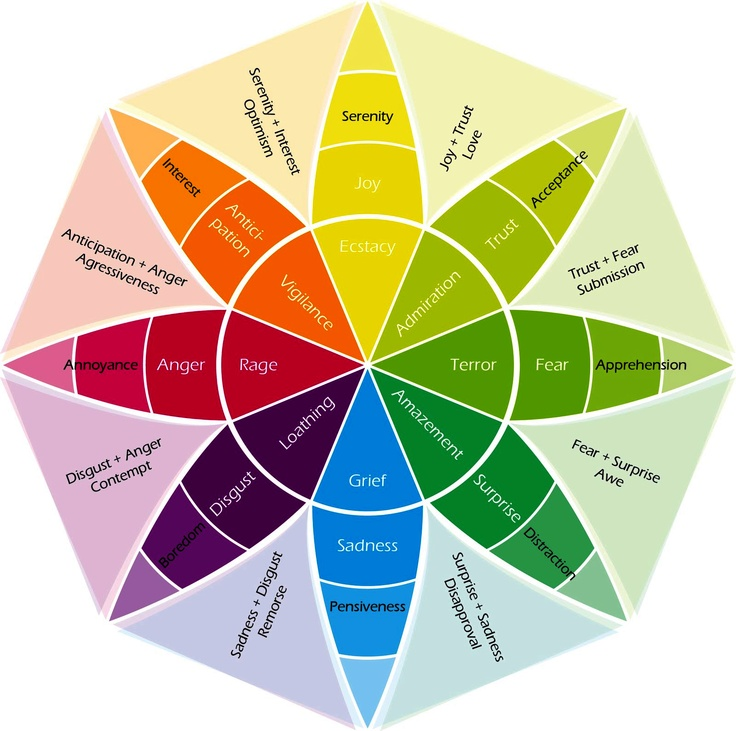
\includegraphics[height=2.56in,width=2.56in]{img/wheel-of-emotions.jpg}
    \caption{Wheel of emotions}
    \label{fig:wheel}
\end{subfigure}
\hfill
\begin{subfigure}[b]{0.45\textwidth}
    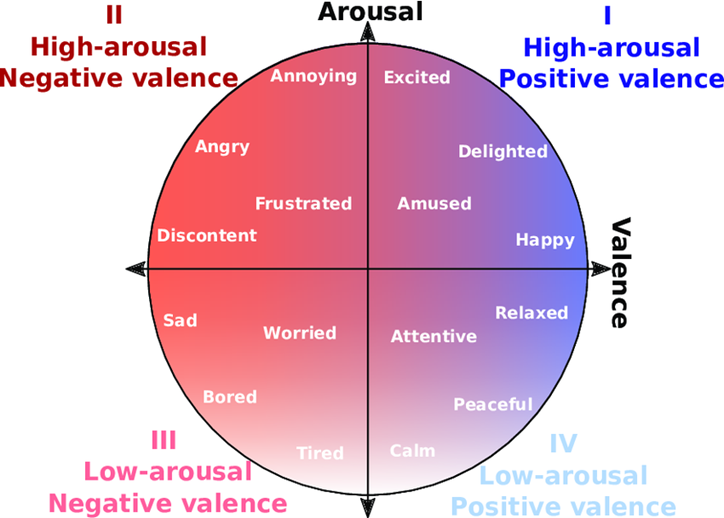
\includegraphics[height=2.4in,width=3.35in]{img/two-dim-modal.png}
    \caption{Russell's two-dimensional model of valence and arousal}
    \label{fig:two-dim}
\end{subfigure}
\caption{Emotion categorization}
\label{fig:combined}
\end{figure*}

\par These emotions are expressed using both verbal and nonverbal channels. As \cite{ekman1971constants} showed, facial expressions universally convey six basic emotions across cultures. Our voices carry emotional information through tone, pitch, and pace, with high-arousal emotions often involving higher pitch and faster pace (Barrett, 2004). Body language, such as posture and gestures, also communicates emotional states \citep{ekman1971constants}. Verbally, we directly express our feelings using linguistic patterns and exact words reflecting higher emotional granularity \citep{smidt2015brief}. In today's digital age, we frequently express emotions in text, a focus of sentiment analysis in natural language processing \citep{lim2016cultural}. Physiological changes like increased heart rate also signal emotions, particularly their arousal levels \citep{barrett2004journal}. 

\par However, the expression of the emotions varies significantly from person to person and across different cultures. Emotional granularity, which is a factor in this variability, is the ability to make fine-grained distinctions between similar emotions \citep{smidt2015brief}. The cultural differences profoundly influence emotional arousal and expression. For instance, research by \citep{lim2016cultural} highlights that Western cultures tend to value and promote high-arousal emotions such as excitement and anger, whereas Eastern cultures prioritize low-arousal emotions like calmness and contentment. Because of that, it’s important to establish a baseline behavior of individuals in advance to identify their emotional state in a more precise manner.

\par Baseline behavior refers to an individual's typical or normal pattern of behavior, thoughts, and emotions when they are not experiencing any specific external stimuli or circumstances that would significantly influence their state. It represents the default or resting state from which deviations or changes can be measured. Emotional baseline, also known as emotional homeostasis or emotional equilibrium, is the relatively stable state of emotional experience that an individual tends to return to after experiencing temporary emotional fluctuations. It is the individual's characteristic or typical level of emotional arousal and emotional experience when not influenced by external events or stimuli. \citep{davidson1998affective} 











